\chapter{Model-based specification}
\label{chapter:specification}

In this chapter, we will look at \emph{model-based specification} --- one style of formal specification. We will look at the \emph{Alloy} language for specification, and how this can be used to describe systems and prove certain properties. In the workshops, we will also look at a tool, called the \emph{Alloy Analyser} for checking properties of Alloy specifications.

\section{What is formal specification?}

Formal specification is the use of mathematical notation to describe properties of a system. The use of mathematical notation provides precision that is not possible with natural language specification, which is subject to ambiguity and incompleteness. Formal specifications provide the specifier with a way to formally define \emph{what} a system must do, without saying \emph{how} it should do it. Thus, they are as formal as a programming language, but they do not constrain the design of the underlying algorithms or data structures.

Because formal specifications do not constrain design detail, and are independent of their implementation, they can be produced early in the project lifecycle; e.g.\ at the requirements and architectural design phases. At these phases, they are particularly valuable. As well as providing an unambiguous reference for system designers and implementers, the mathematical nature of formal specifications provides software engineers with the opportunity to \emph{prove} properties about the specification, such as correctness, completeness, and consistency, but also other properties, including safety and security.

In this chapter, we will use the \emph{Alloy} specification language. Alloy is based on the Z language, which is the most widely used and probably widely known formal specification language. Alloy sacrifices the expressiveness of Z for computational tractability; that is, some expressive features in Z are removed to allow us to automatically check properties of Ally specifications.

In this subject, we use Alloy for two reasons:

\begin{enumerate}
 \item It offers an intuitive notation.
 \item The Alloy Analyser tool for checking Alloy specifications is a state-of-the-art research prototype, which has been applied to many problems, and is supported by a large community of users.
\end{enumerate}


\section{What is model-based specification?}

Model-based specification is an approach to formal, system specification in which the system is defined as a state machine model. That is, there is a state representing the data in the system, and operations specify the transitions that can take the system from one state to another. This is much like the idea of a module/package in Ada: the variables define the state, and the subprograms define the transitions. The clean mapping from model-based specifications to modules is one reason that model-based specification has become the preferred method for formal specification, as opposed to axiomatic or algebraic approaches, which specify the properties of the systems via sets of axioms.

\paragraph{Model-based specification in the software engineering lifecycle.}
Model-based specification is not a requirements elicitation technique, nor is it generally a requirements engineering technique. Many model-based specifications are finalised during architectural design, once the components of the system are known. However, the formalisation of the behaviour of system components implicitly leads to a formalisation of those system requirements that the components are implement. As such, model-based specification falls over the phases of requirements engineering and architectural design. We should be comfortable with this, as in modern software engineering, the line between requirements and architectural design is blurred.

Figure~\ref{fig:specification:sdlc}, adopted from Sommerville \cite[Ch.\ 27]{sommerville10} shows the relationship between different activities in the early software engineering phases, and how model-based specification is typically carried out in parallel with other activities. Information flow between the activities is two-way --- information is always passed between the requirements and design phases.

\begin{figure}[!h]
\centering
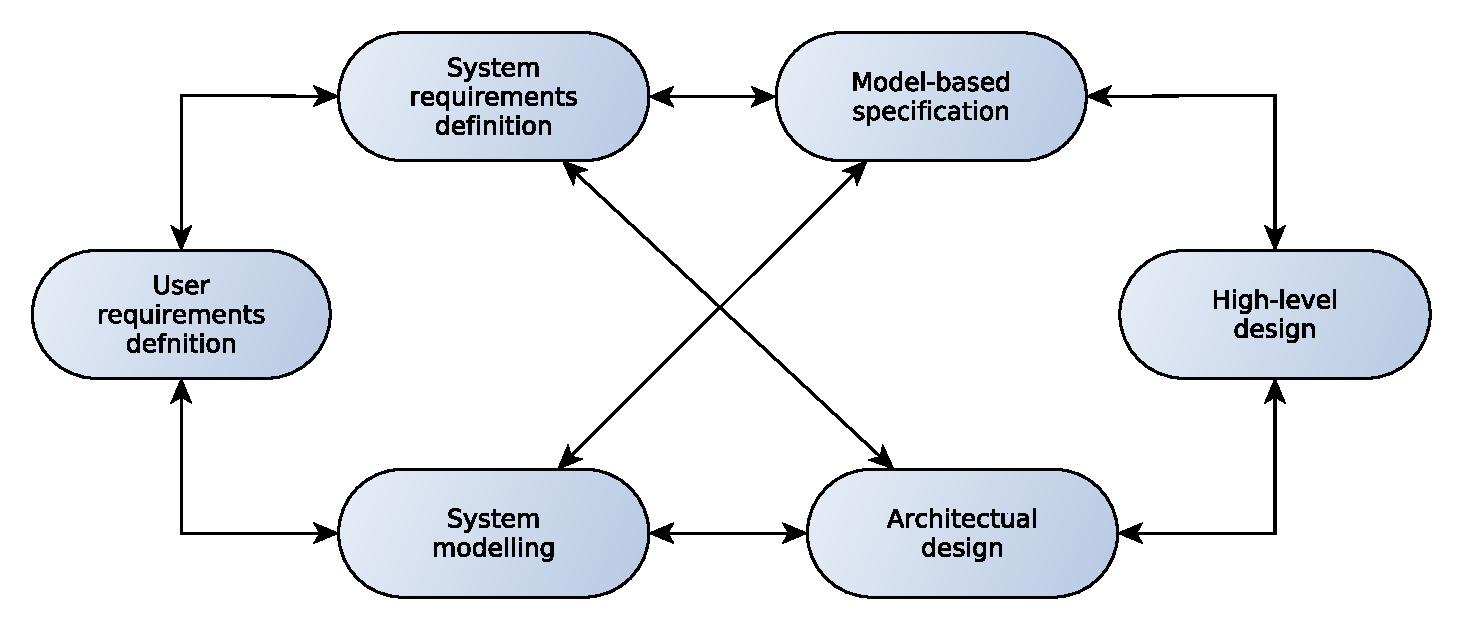
\includegraphics[scale=0.6]{\rootdir/specification/figures/specification-in-lifecycle}
\caption{Model-based specification in the software process.}
\label{fig:specification:sdlc}
\end{figure}

\paragraph{Languages for model-based specification.}
There are several well-known languages for model-based specification, including VDM, B, Z, and Alloy. These languages all have commonalities, especially that data types are based on sets and relations, and operations are specified using predicate logic. UML statecharts are another example of model-based specification, although the level of formality in these is less than in VDM, B, Z, and Alloy, as the intended areas of use are different.

\paragraph{Model-based specification and natural language.}
Like programming languages, formal, model-based specifications cannot be understood fully by a simple read over. As such, documenting the specification using natural language is important, just like commenting program code. Natural language descriptions not only allow the reader to understand the specification at a superficial level without having to worry about detail, but also allow the reader to understand the formal details, by guiding them through the meaning.


\section{The costs of formal specification}
\label{sec:specification:costs}

Using a rigorous process and method for formally specifying system properties is clearly a costly exercise. The activity of specifying the precise detail of systems and sub-systems using mathematical notation requires careful thought and increased knowledge about the systems. Further, they must come under the same scrutiny of quality assurance using reviews and inspections as other requirements specification techniques. 

The question to be asked is: \emph{``Is the cost worth it?''}.

A major limitation to formal specification, even in high integrity domains, is that the cost is too high. However, studies repeatedly show the following: the cost of specification is higher, but some of the added costs are recouped later in the process. Figure~\ref{fig:specification:costs-of-formal-specification}, taken from from Phillips \cite{phillips89}, shows data from a project, comparing the number of errors found per thousand lines of code of using the Z specification language, against not using formal specification at all. The project from which the data comes from is the CICS project undertaken at IBM. The project introduced 268,000 lines of new code into a system already containing 500,000 lines of code. Of the new code, 48,000 lines was engineered from a formal specification written in Z. Z was used at the product-, component-, and module-level design stages.

\begin{figure}[!h]
\centering
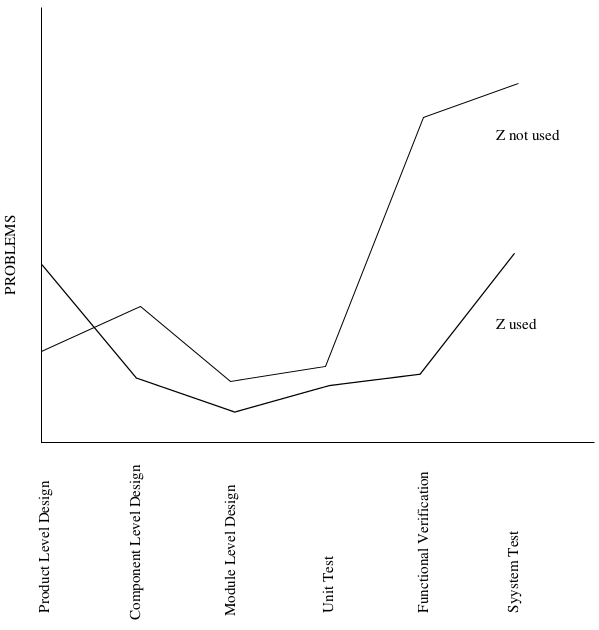
\includegraphics[scale=0.6]{\rootdir/specification/figures/CICS-graph}
\caption{The costs of formal specification on the CICS project.}
\label{fig:specification:costs-of-formal-specification}
\end{figure}

Let's analyse this figure and ask ourselves why formal specification would \emph{reduce} the costs of later phases. There are a number of reasons for this:

\begin{enumerate}
 \item Using mathematical notation removes ambiguity from specifications, which is a cause of many problems in software. This helps to limit the amount of re-work in later phases, driving down their costs.

 \item Some cost incurred during design and implementation is simply trying to decide exactly what the behaviour of the system could be. Using natural language to specify requirements means that we can be shorthanded and therefore miss important detail. Using mathematical notation does not afford this because it is easy to show incompleteness, and many of the issues that generally present themselves during design and implementation must be solved during specification instead. In other words, the people doing the specification do some of the work typically undertaken at the design and implementation phases.


 \item Despite opinion to the contrary, designing and implementing a system from a formal specification is \emph{more} straightforward than doing so from natural language requirements. For a novice, this may not be the case, but for someone who is as comfortable with mathematical notation as they are with programming languages, this is most definitely the case.

 \item Using formal notation offers the possibility of \emph{proving} that our specification satisfied certain properties. Discovering in later phases that our specification does not satisfy some properties is more costly than discovering these in early phases.

 \item Post-release costs are reduced due to the fact that less mistakes are introduced over the process; or more accurately, the same number of mistakes are made, but more are made \emph{and found} during specification, rather than post release.
\end{enumerate}

A simple (and common) objection to formal specification is that it is just too hard: the formality is too difficult for the average programmer to grasp. I agree that this is case. I would not advocate employing formal specification on a project with programmers who have no experience at it. However, I disagree that this \emph{has to be} the case. The average programmer is already intelligent enough to have learnt a formal language: all programming languages are formal. As such, we know they are equipped to deal with formal languages, even at the specification language. 

However, an important extension to this argument is the following: \emph{formal specification is much simpler than programming --- we only have to specify \emph{what} a system should do, whereas our program must specify \emph{how} to do it}.

If programmers were trained in formal specification languages the same way they were trained in programming languages, reading and using formal specifications would not be an issue. Thus, the cost of formal specification would be \emph{significantly} less than the cost of implementation.

That is not to say that formal specification should be used in every organisation or on every project: it is only cost effective when the cost of releasing software with faults is greater than the cost of preventing them. In environments where the biggest issue is responding to change (e.g.\ change of customer preferences, change of requirements from a client), ensuring the software is correct is not as high of a priority as getting something out that works for most normal cases.

In high integrity systems, formal specification is generally only applied to those parts of the system that contain high-integrity requirements. Other parts of the system, for example, data storage or user interface, are engineered using more standard techniques.

\section{Logic and set theory}

Sum is based on \emph{first-order predicate logic} and \emph{set theory}; both topics with which all students in this subject are expected to be familiar. 
The set theory part of Sum contains the standard set theoretic concepts, such as set comprehension, power sets, set operators (union, intersection, subset, etc.), Cartesian products, relations, and functions. The predicate logic part of Sum contains propositional operators (``and'', ``or'', ``implies'', etc.) and existential and universal quantifiers (``for all'', ``there exists'').

The most important concepts with which you are expected to be familiar are:

\begin{itemize}

 \item First-order logic: conjunction (``and''), disjunction (``or''), implication, negation, universal quantification (``for all''), and existential quantification (``there exists'').

 \item Set theory: set membership, set comprehension, set union, set intersection, set difference, and subsets.

 \item Relations: Cartesian product, domain and range of relations, sequences, partial functions, and total functions.

\end{itemize}

If you are not familiar these concepts, or the details are hazy, Chapter 3 of Daniel Jackson's book \emph{Software Abstractions: Logic, Language, and Analysis}, provides a detail description of these concepts, and how to express them in Alloy.

If you cannot access this, Chapters 2-9 in Woodcock and Davies book ``Using Z'' \cite{woodcock-using-z} provides a detailed description of basic logic and set theory, which can also be read lightly to pick up the most important aspects. A PDF version of this book is available on the LMS for download.

\subsubsection{Why sets and predicates?}

Most model-based languages are based on sets and predicates. The reasons are quite simple: 

\begin{enumerate}

 \item Set theory (sets, relations, functions, etc.) provides us with enough notation to specify the data of any system. Just as importantly though, it \emph{restricts} us from specifying design detail, and force us to think more abstractly --- something which is important at the specification level. 

 \item Predicate logic provides us with sufficient expressive power to specify what changes the data of a system can undergo over time (or the effect of operations on data). Just as importantly, it \emph{restricts} us from specifying \emph{how} those changes should be implemented.

These first two points are important: requirements engineering is already difficult enough without us thinking about design and implementation problems at the same time.

 \item Together, proof theory and understanding of set theory and predicate logic is strong enough that we can prove many properties specified using these parts. We can take advantage of hundreds of years of work in these areas and apply this to software engineering --- a field that is relatively new in comparison.

\end{enumerate}


\begin{example}
As an example of using logic and set theory to specify software and system behaviour, and how this differs from programming, consider the trivial example of sorting a list of integers.

To specify the behaviour of a procedure that takes a (possibly unsorted) list and sorts it, we have to say that:

\begin{enumerate}

 \item each element in the input list is present in the output list (that is, the output list is a permutation of the input list); and

 \item each element of the output list is less than or equal to the next (that is, the list is sorted).

\end{enumerate}


We can specify what it means for a list of integers to be sorted:
\[
 \forall list : \seq \integer @ ~~sorted(list)~~ \iff~~  \forall i : 1 \upto \#list - 1 @ list(i) \leq list(i + 1)
\]
This states that, for all sequences of integers, that sequence is sorted \emph{if and only if}: for each index (except the last) in the list, the integer at that index is less than or equal to the integer at the next index.

We can also specify what it means for one list to be a permutation of the other.
\[
 \forall a, b : \seq \integer @  ~~permutation(a,b)~~ \iff~~  \forall el : \integer @ count(el, a)  = count(el, b)
\]
 
in which $\mathit{count}$ is defined as:
\[
 \forall el : \integer; list : \seq \integer; c : \nat @~~ count(el, list) = c ~~\iff~~
    c = \#(list\rres \{el\})
\]

That is $count(el, list) = c$ if and only if $c$ is the number of elements when we take the \emph{range restriction} of $list$ on $el$ only.

Finally, we can specify the precondition and postcondition of a procedure using these concepts:

\textbf{procedure}  $sort (in\_list : \textbf{in} \seq \integer; out\_list : \textbf{out} \seq\integer)$ \textbf{is}

\vspace{-2mm}

\quad \textbf{pre} ~$\#in\_list > 1$

\vspace{-2mm}

\quad \textbf{post} $sorted(out\_list) \land is permutation(in\_list, out\_list)$

Here, we have added a superficial precondition that the list is not empty.

So, this example specifies the functional behaviour of sorting a list, but does NOT specify \emph{how} the list should be sorted. Any correct algorithm for sorting integers will suffice to fulfil the specification above.

\end{example}

\begin{example}
Using the definitions above, we can specify the behaviour of a binary search algorithm in a straightforward manner:

\textbf{procedure}  $binary\_search (list : \textbf{in} \seq \integer; target : \textbf{in}\ \integer; index : \textbf{out}\ \integer)$ \textbf{is}

\vspace{-2mm}

\quad \textbf{pre} ~$sorted(list)$

\vspace{-2mm}

\quad \textbf{post} $target = list(index) \lor (target = -1 \iff target \notin \ran(list))$

In this example, we have called the procedure ``$binary\_search$'', but only because we specify in the precondition that the input list must be sorted. Other than this, the algorithm is not constrained by any particular binary search algorithm (e.g.\ recursive or iterative), and in fact, does not truly constrain it to a binary search algorithm at all.

We can see from this example: specifying binary search behaviour is much neater than specifying the algorithm to achieve it.

\end{example}

\section{The Alloy language}

In this chapter, we will present the Alloy language. We will present only a small subset of the language, but it is enough of a subset to allow specification of state models. The Alloy has a rich notation for combining predicates, which allow flexible and incremental building of specifications. We will not go into detail on all of these operators, but we will use some of the basic components to enable clean specification.

An Alloy reference manual is available online at:

 \url{http://alloy.mit.edu/alloy/documentation/book-chapters/alloy-language-reference.pdf}

 It provides detailed syntax and semantic definitions. 

\subsection{Types and sets}

Sum is a \emph{typed} language, which means that all variables have a type. The type system for Sum is very simple: a type is a set. Therefore, a declaration \texttt{x : S}, where \texttt{x} is the variable and \texttt{S} is the type, is simply saying that \texttt{x} is in the set \texttt{S}. The set \texttt{S} can be used as an expression in predicates as well, for example \texttt{T = S}, which says that the two sets \texttt{S} and \texttt{T} are equal.

There are only three basic types in Sum: the set of integers, called \texttt{int}; the set of characters, called \texttt{char}; and the set of strings, called \texttt{string}. Other types are built from these, including the set of natural numbers, \texttt{nat}. More complex types can be built up using Cartesian products and finite/power sets. For example, the set \texttt{int cross int}, where \texttt{cross} is the Cartesian product operator, defines the set/type of all pairs of integers.

\begin{example}
To declare a variable, \texttt{x}, of a set of integers, we would use:

\quad\quad \texttt{x : power int}

in which \texttt{power} is a keyword used to represent the powerset operator. Thus, the set \texttt{power int} is the set of all sets of integers, and \texttt{x} is an element of this set, meaning that the type of \texttt{x} is a set of integers.

\end{example}

\begin{example}
To declare a variable, \texttt{y}, of a pair of integers, we would use:

\quad\quad \texttt{y : int cross int}

The set \texttt{int cross int} is the set of all pairs of integers, and  \texttt{y} is an element of this set, meaning that the type of \texttt{y} is a pair of numbers. If we wanted to declare a pair in which the first element is an integer, and the second is a set of integers, we could use:

\quad\quad \texttt{y : int cross power int}

\end{example}

We can declare a variable to be in a particular set, but its type remains as the maximal set of that type. That is, if we have the declaration:

\quad\quad \texttt{x : \{1,2,3,4,5\}}

the \emph{type} of \texttt{x} is still an integer, however, its \emph{value} can only be in the range \texttt{1 .. 5}. This means that the for the declarations \texttt{x : nat} and \texttt{x : int}, the type of \texttt{x} is the same (integer), but the values it can take on differ.

\subsubsection*{Declaring new basic types}

New basic types can be declared in a specification. There are two ways new basic types can be declared. The first is a \emph{given type}, which can be declared as follows:

\quad\quad \texttt{[}\emph{GivenType}\texttt{]}.

This introduces a new type called \emph{GivenType}, whose internal structure is invisible. It also introduces a new infinite set called \emph{GivenType}. There are no concrete values for this set. This is fine for a specification, because we are interested in abstracting the domain, and some details about types and sets may be irrelevant.

\begin{example}
\label{ex:specification:customer-given-type}
Consider a system that keeps track of the customers  entering and leaving a bakery. In this system, the details of the customer, such as name, age, height, etc., are irrelevant, because all we want to know is the set of customers that are in the store. As such, we may declare a new type called \texttt{Customer} as follows:

\lstset{aboveskip=3mm}
\begin{lstlisting}
  [Customer];
\end{lstlisting}

We can declare a variable of type customer; e.g. \texttt{c : Customer}, or a set of customers (\texttt{sc : power Customer}), but we cannot see concrete values of \texttt{Customer}.

\end{example}

The other way of declaring new types is to use \emph{free types}. Free types are similar to given types, except that concrete values must be provided. A free type is declared as follows:

\quad\quad \emph{FreeType} \texttt{::=} \emph{value1} \texttt{|} \emph{value2} \texttt{|} \ldots

This introduces a new type called \emph{FreeType}, which can have values from the set \texttt{\{value1, value2,} \ldots \texttt{\}}, and which can \emph{only} have values from that set. It also declares the set called \emph{FreeType}. Further to this, it introduces the constants \texttt{value1}, \texttt{value2}, etc.\ into the specification, and also specifies that \texttt{value1}, \texttt{value2}, etc.\ are all \emph{distinct} from one another.

\begin{example}
\label{ex:specification:colour-free-type}
Consider a system that needs to keep track of a finite set of known colours. We can declare a free type called \texttt{Colour} as follows:

\lstset{aboveskip=3mm}
\begin{lstlisting}
  Colour ::= red | yellow | pink | green | purple | orange | blue;
\end{lstlisting}

The declaration \texttt{c : Colour} declares \texttt{c} to be of type \texttt{Colour}, but further to that, in the specification we can use the names of the colours in predicates, such \texttt{c = red}, to signify that the value of colour \texttt{c} is \texttt{red}.

\end{example}

Free types actually support more complex (and recursive) type definitions, however, for the purpose of this subject, the above syntax is sufficient.

As with the basic integer type, given types and free types can be used to construct more complicated types. For example, if we are selling coloured shirts and want to keep track of the number of each colour, we could declare the variable \texttt{colour\_count} as follows:

\begin{lstlisting}
  colour_count : power(Colour cross nat)
\end{lstlisting}

where \texttt{power(Colour cross nat)} describes the set of sets of all pairs of colours and natural numbers.

However, it would be more succinct to declare this as a \emph{function} (in the set theoretic sense), as follows:

\begin{lstlisting}
  colour_count : Colour --> nat
\end{lstlisting}

where \texttt{-->} is the function arrow. This is a neater declaration because the above declaration is the same as \texttt{power(Colour cross nat)}, except that each colour is mapped to exactly one number.

\subsection{Modules}

The basic unit of modularity in Sum are \emph{modules}. Modules are the main difference between Z and Sum. A module is declared with the format:

\lstset{language=}
\lstset{aboveskip=3mm}
\begin{lstlisting}[escapeinside={||}]
  module |\emph{ModuleName}| is
    |\ldots|
  end |\emph{ModuleName}|
\end{lstlisting}

\subsection{State}

A module can have a \emph{state}. The state specifies the variables of the specification, their types, and the legal values that these variables can have. A Sum state specification is declared with the format:

\lstset{aboveskip=3mm}
\begin{lstlisting}[escapeinside={||}]
  schema state is
  dec
    |\emph{Variable declarations}|
  pred
    |\emph{State invariant predicate}|
  end state;
\end{lstlisting}

The keyword \texttt{dec} is short for ``declaration'', and the keyword \texttt{pred} is short for ``predicate''. The predicate part of the schema is the \emph{state invariant}. This means that all of the operations in the specification (we will see these later), must preserve this invariant.

\begin{example}
 Let consider an example of a simple toy specification of a bakery. In the bakery, customers can arrive, be served, and leave. The state of the specification keeps track of the customer that are currently in the bakery, and the customer that is currently being served (if any).

The state for the bakery can be described as follows:

\lstinputlisting[linerange={5-12}]{\rootdir/specification/code/bakery.sum}

\end{example}

\texttt{Customer} is the set of customers, as declared in Example~\ref{ex:specification:customer-given-type}.  This state schema declares that there are two variables: \texttt{in\_shop} and \texttt{being\_served}, and both are sets of customers. They represent the set of customers in the shop, and the set of customers being served.

 The invariant states that there is at most one customer being served at any time, and that the customer being served is in the shop.


\subsection{Operations}

Operations specify the allowed transitions between states of the system. They are constructed using declarations and predicates, similar to that of the state schema, except that they also permit input and output variable declarations.

The syntax of an operation declaration is as follows:

\lstset{aboveskip=3mm}
\begin{lstlisting}[escapeinside={||}]
  op schema |\emph{OperationName}| is
  dec
    |\emph{Variable declarations}|
  pred
    pre |\emph{Precondition predicate}|;
    |\emph{Postcondition predicate}|;
    changes_only {|\emph{List of state variables}|}
  end |\emph{OperationName}|;
\end{lstlisting}

\textbf{Note:} The semi-colon at the end of the listing above signifies \emph{composition}, meaning that a list of operations can be declared, and they are composed together to form a single module specification. However, the \emph{last} operation specified in a module should terminate \emph{without} a semi-colon, because it is not composed with another operation.

The variable and the type declarations are input variables, output variables, or local variables. To distinguish these, the variable names for input variables should be suffixed with a question mark (e.g.\ \texttt{in?}), output variables with an exclamation point (e.g.\ \texttt{out!}), and local variables should be suffixed with  neither. 

State variables (that is, those declared in the state schema) are implicitly declared. Specifically, there are \emph{two} versions of every state variable declared: one that refers to the value of the variable \emph{before} the operation is executed; and one that refers to the value \emph{after} the operation has executed (called the \emph{post-state} value). The post-state variable is distinguished from the pre-state variable using a single quote mark (e.g.\ \texttt{in\_shop'}).

The predicate part of the operation specifies the behaviour. It is broken into three parts:

\begin{itemize}
 \item The \emph{precondition}: Specifies a predicate that must hold for the operation to be \emph{enabled}. If this precondition is false, the behaviour of the operation is undefined.

 \item The \emph{postcondition}: Specifies the predicate that must hold after the operation has been executed, and provided that the precondition was true.

 \item The \emph{variable change set}: Specifies the state variables that can be changed by this operation. This is known as the \emph{frame}. If a state variable, \texttt{v}, is in \emph{not} in the change set, then the predicate  \texttt{v' = v} is implicitly added to the postcondition. If a state variable is in the change set, but is not referred to in the postcondition, its value is unconstrained, meaning that it can take on any legal value.

\end{itemize}

\begin{example}
The best way to demonstrate operations is via an example. We'll use our earlier example of customers entering and leaving a bakery. 

The \texttt{Arrive} operation models the behaviour of a new customer entering the bakery. Recall that the state variable \texttt{in\_shop} models the set of customers entering the shop. The \texttt{Arrive} operation should therefore add the new customer to the set of customers in the shop, while not changing the set of customers being served:

\lstinputlisting[linerange={20-29}]{\rootdir/specification/code/bakery.sum}


The customer variable, \texttt{c?}, specifies the input: the customer entering the bakery. The precondition is that the customer is not already in the bakery; that is, a customer already in the bakery should bot be able to enter twice --- corresponding to our expectations that humans cannot alter the space-time dimension and be in two places at once.

To add the customer to the set of customers in the shop, set union is used:

\quad\quad \texttt{in\_shop' = in\_shop union \{c?\}}

The states the the post-state value of \texttt{in\_shop} is equal to the pre-state value with \texttt{c?} added.

\end{example}

\textbf{Note:} A postcondition is a predicate: an assertion about the world (or about the state). It is \emph{not} a program statement. As such, we cannot have multiple postconditions updating the same variable. For example, if the \texttt{Arrive} operation had two inputs, \texttt{c1?} and \texttt{c2?}, the predicate:

\quad\quad \texttt{in\_shop' = in\_shop union \{c1?\};}

\vspace{-2mm}

\quad\quad \texttt{in\_shop' = in\_shop union \{c2?\};}

could not be used. In fact, this predicate only has a solution if \texttt{c1? = c2?}, because the lines above must hold \emph{simultaneously}. This is an important part of the language, because it constrains us to saying \emph{what} the behaviour should be, while restricting our ability to say \emph{how} is should be achieved.

\begin{example}
As an additional example, let's consider the the operation for customers leaving the bakery:

\lstinputlisting[linerange={42-50}]{\rootdir/specification/code/bakery.sum}

To leave, a customer must already be in the shop, so this is the precondition. The postcondition specifies that if the customer leaves, then they are no longer being served, and are no longer in the shop. The \texttt{diff} operator is just the ``set difference'' operator.

\end{example}

\subsection*{Non-determinism}

For some predicates, there may be more than one solution (bindings of values to variables) for a given input to an operation. This is known as \emph{non-determinism}, because the output cannot be uniquely determined. As an example, consider the following operation, \texttt{Serve}, in which a customer is chosen to be the one being served in the bakery:

\lstinputlisting[linerange={31-40}]{\rootdir/specification/code/bakery.sum}

In this operation, the output variable \texttt{c!} displays the new customer being served. The precondition specifies that no other customer should be served at the time. The postcondition specifies that the new customer must be selected from those already in the shop, and that they must be now in the \texttt{being\_served} set.

However, note that if there is more than one customer in the shop (that is, the set \texttt{in\_shop} has more than one element), then the variable \texttt{c!}, and as a result the set \texttt{being\_served'} can have more than one possible value. Therefore, this operation is non-deterministic.

Non-determinism is valuable in specification, because often we may want to say that a range of solutions are possible, but we do not care which solution is chosen. In addition, this also provides us with an abstraction mechanism. If we are forced to provide a single solution, this may further force us to specify \emph{how} the solution must be arrived at.

\subsection{The \texttt{init} operator}

A Sum specification can contain a special operator called \texttt{init}, which is the operator that \emph{initialises} the module. Unlike operation schemas, which implicitly include pre- and post-state variables, the \texttt{init} schema has only post-state variables, because it will initialise the module, so cannot have pre-state values. The \texttt{init} schema must always be named ``\texttt{init}''.

An \texttt{init} operation schema must be declared using the following syntax:
\lstset{aboveskip=3mm}
\begin{lstlisting}[escapeinside={||}]
  schema init is
  dec
    |\emph{Variable declarations}|
  pred
    |\emph{Postcondition predicate}|;
  end init;
\end{lstlisting}

Note that there is no \texttt{op} keyword used for the initialisation schema.

\begin{example}
For bakery example, the \texttt{init} schema specifies that there are initially no customers in the shop and no customers being served:

\lstinputlisting[linerange={14-18}]{\rootdir/specification/code/bakery.sum}

\end{example}

\subsection{Other paragraphs}

As well as modules, state schemas, and operations, Sum specifications can contain other types of paragraphs. In this section, we present just a handful of the most useful and relevant.

\subsubsection*{Abbreviations}

Abbreviation paragraphs allow us to assign an expression to a name, which can improve readability and also make the task of specification more straightforward. The syntax for an abbreviation is:

\lstset{aboveskip=3mm}
\begin{lstlisting}[escapeinside={||}]
  |\emph{Name}| == |\emph{Expression}|;
\end{lstlisting}

This will introduce a new variable called \emph{Name}, which will have the value \emph{Expression}. The type of \emph{Name} will be the same as the type of \emph{Expression}

An abbreviation is analogous to a constant definition. The variable is not a state, input, output, or local variable, and its value cannot change.

\begin{example}
Recall the use of the free type \texttt{Colour} in Example~\ref{ex:specification:colour-free-type}. This introduces the type and set \texttt{Colour}, as well as several colour names.

If we want to have the set of just primary colours, we could use an abbreviation paragraph:

\lstset{aboveskip=3mm}
\begin{lstlisting}
  PrimaryColours == {red, yellow, blue};
\end{lstlisting}

Note that the names \texttt{red}, \texttt{yellow}, and \texttt{blue} need to have been declared as well.

The type of \texttt{PrimaryColours} is \texttt{power Colour}. 

\end{example}


\subsubsection*{Axiomatic definitions}

Axiomatic definitions allow us to introduce new terms into the specification, but with constraints on them. These new terms are constant variables, as with abbreviations, but can be more than simple abbreviations.

The syntax for an axiomatic definition is:

\lstset{aboveskip=3mm}
\begin{lstlisting}[escapeinside={||}]
  axiom is
  dec    
    |\emph{Variable declaration}|
  pred
    |\emph{Predicate}|
  end
\end{lstlisting}

The predicate part of the axiom constrains the value of the variables declared.

\begin{example}
Recall that in Sum, the only declared basic type is \texttt{int}. The set of natural numbers is defined using an axiomatic definition:

\lstset{aboveskip=3mm}
\begin{lstlisting}
  axiom is
  dec    
    nat : power int
  pred
    forall x : nat @ x >= 0
  end;
\end{lstlisting}

This introduces a new name \texttt{nat} into the specification, which is the set of integers that are all greater than or equal to 0.

\end{example}

\begin{example}
Axiomatic definitions can be more than simple types: they can be relations or functions. The following example defines a function for calculating the square of a number:

\lstinputlisting[caption={Axiomatic definition for squaring a natural number (\textbf{square.sum})}]{\rootdir/specification/code/square.sum}

This defines a \emph{total function} between a natural number and its square. Thus, it is a static structure that can be visualised as follows:

\begin{center}
 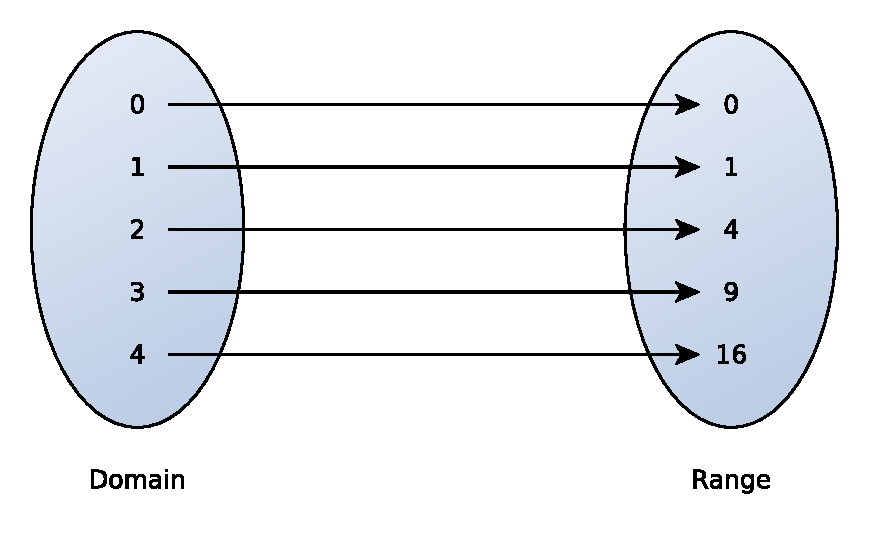
\includegraphics[scale=0.7]{\rootdir/specification/figures/square-function}
\end{center}

The domain of the function is on the left (the natural numbers) and the range is on the right (also the natural numbers).

\end{example}

\subsubsection*{Generic definitions}

Axiomatic definitions can be \emph{generic}. A generic definition is the same as an axiomatic definition, but the type of at least one of the declared variables is generic, which means that the definition declares a family of constants. 

The syntax for a generic definition is the same as for an axiomatic definition, except that the generic parameters must be declared:

\lstset{aboveskip=3mm}
\begin{lstlisting}[escapeinside={||}]
  axiom[|\emph{Generic Parameter List}|] is
  dec    
    |\emph{Variable declaration}|
  pred
    |\emph{Predicate}|
  end;
\end{lstlisting}


\begin{example}
We can introduce a constant called \texttt{emptyset}, which is defined as a set containing nothing:

\lstset{aboveskip=3mm}
\begin{lstlisting}
  axiom[X] is
  dec    
    emptyset : power X
  pred
    emptyset = {}
  end;
\end{lstlisting}

We can use this symbol in a predicate such as \texttt{\{1\} = emptyset} (which will evaluate to false), or \texttt{\{red\} = emptyset} (which would also evaluate to false). However, if we had declared \texttt{emptyset} to be of type \texttt{power int}, then the predicate \texttt{\{red\} = emptyset} would have a type inconsistency, because the type on the left of the equality is \texttt{power Colour}, while on the right the type would be \texttt{power int} --- an inconsistency.

\end{example}

\begin{example}
As with axiomatic definitions, generic definitions can be used to define relations and functions. A relation \texttt{issubset} can be defined as follows:

\lstinputlisting[caption={Generic definition for a subset relation (\textbf{subset.sum})}]{\rootdir/specification/code/subset.sum}

This is a relation between two sets of \texttt{power X}, where \texttt{X} is the generic parameter that must be instantiated; e.g. in the predicate \texttt{issubset(\{1,2\}, \{1,2,3\})}, \texttt{X} would be instantiate to \texttt{int}.

\end{example}

Abbreviations, axiomatic definitions, and generic definitions can be declared inside modules, and would then become attributes of that module, or they can be declared outside of modules, and they are then global.

\subsection{Schemas}

\subsubsection{Schemas as sets/types}

We have already seen schemas: they are used to specify the state and operations of a module. However, schemas can also be used as types and sets. Using a schema as a type, we can introduce \emph{compound} types, analogous to the record types in Ada, or structs in C.

As with other types, this also introduces a set, as well as a type. The difference between the compound types found in programming languages and schema types in Sum is that the values of the types can be constrained by schema types.

\begin{example}
As an example, consider the compound type of \texttt{Date}, as defined using Ada records in Section~\ref{sec:ada:defining-new-types}. In Sum, we can define a type \texttt{Date} using the following:

\lstset{aboveskip=3mm}
\lstinputlisting{\rootdir/specification/code/date.sum}

Thus, the set \texttt{Date} contains a list of dates that correspond to the predicate above. As such, if we have a variable, \texttt{date}, of type \texttt{Date}, in which the date represents the 29 Feb, 2013, the predicate \texttt{date in Date} would be false.

\end{example}

Expressions that are of a schema type are known as \emph{binding extensions}. They are of the format:

\lstset{aboveskip=3mm}
\begin{lstlisting}[escapeinside={++}]
  <|+\emph{Var1}+ == +\emph{Expression1}+, +\emph{Var2}+ == +\emph{Expression2}+ , +\ldots+ |>
\end{lstlisting}

\begin{example}
The following two predicates hold:

\begin{lstlisting}
  <|day == 1, month == 1, year == 2013|> in Date
  <|day == 29, month == 2, year == 2013|> not_in Date
\end{lstlisting}

\end{example}

We can refer to the sub-component of the binding expression using the syntax:


\lstset{aboveskip=3mm}
\begin{lstlisting}[escapeinside={++}]
  +\emph{Expression}+.+\emph{Var}
\end{lstlisting}

in which \texttt{Expression} is an expression of type schema, and \texttt{Var} is a variable declared in that schema.

\begin{example}
~

\lstset{aboveskip=3mm}
\begin{lstlisting}
  axiom is
  dec
    assignment_1_due_date : Date
  pred
    assignment_1_due_date.day = 27;
    assignment_1_due_date.month = 3;
    assignment_1_due_date.year = 2013
  end
\end{lstlisting}

\end{example}

\subsubsection{Schemas calculus}
\label{sec:specification:sum:schema-calculus}

Inherited from Z, Sum has a rich schema calculus that allows schemas to be combined. In this section, we present just a small part of this calculus, but enough to enable clean and readable specification using Sum.

\subsubsection*{Schemas as declarations}

Schemas can be included as declarations in other schemas. The syntax for this is:

\lstset{aboveskip=3mm}
\begin{lstlisting}[escapeinside={||}]
  schema |\emph{LargeSchema}| is
  dec
    |\emph{Schema1}|;
    |\emph{Schema2}|;
    |\ldots|
  pred
    |\emph{Predicate}|
  end |\emph{LargeSchema}|;
\end{lstlisting}

The inclusion of schemas into the declaration part of the new schema has two effects:

\begin{enumerate}
  \item it includes the declarations from both schemas into the declaration of the new schema; and
  \item it includes the predicates from both schemas into the predicate of the new schema, and conjoins them into a single predicate.
\end{enumerate}

Therefore, it is semantically equivalent to taking the included schemas, copying the declarations into the declarations of \emph{LargeSchema}, and the copy the predicates into the predicate part of \emph{LargeSchema}.

\begin{example}
Consider the following example from Sommerville \cite{sommerville10} of a storage tank in a chemical processing plant:


\lstinputlisting[linerange={3-9}, caption={The \texttt{Container} schema}, label={listing:specification:container}]{\rootdir/specification/code/storage.sum}


The container has a maximum capacity (for example, in litres), and a current contents. The contents must not exceed the capacity.

Now consider a component of an indicator light for alerting someone of a dangerous situation:

\lstinputlisting[linerange={11-20},caption={The \texttt{Indicator} schema}, label={listing:specification:indicator}]{\rootdir/specification/code/storage.sum}


These two building blocks can be combined into a larger component. For example, having introduced the \texttt{Container} and \texttt{Storage} schemas, we can now create the state of a module using them:

\lstinputlisting[linerange={22-30},caption={The state schema for the \texttt{Storage} module, which links the container and indicator building blocks}, label={listing:specification:storage}]{\rootdir/specification/code/storage.sum}

Semantically, this is exactly equivalent to the following:

\lstset{aboveskip=3mm}
\begin{lstlisting}[caption={The expanded version of the state schema for the \texttt{Storage} module}, label={listing:specification:storage-expanded}]
  schema state is
  dec   
    contents : nat;
    capacity : nat;
    light : Light;
    reading : nat;
    danger_level : nat
  pred
    contents <= capacity ;
    light = on <=> reading <= danger_level;
    reading = contents;
    capacity = 5000;
    danger_level = 50
  end state
\end{lstlisting}

So, the inclusion of the two schemas brings them together. In the ``new'' predicate part, the predicate \texttt{reading = contents} links to two together, specifying that the reading should be obtained from the contents, and semantically, this states that the light should come on if the contents are a specified danger level (in this case, 50).

\end{example}

Although the two schemas in Listings~\ref{listing:specification:storage} and \ref{listing:specification:storage-expanded} are semantically equivalent, the former is arguably more readable. Further, schema inclusion provides better support for the ``divide and conquer'' approach to software engineering, in which the problem is broken down into smaller, more manageable problems, and then brought back together.

\textbf{Note:} When using schema inclusion, if more than one schema is included in the declaration part, the types of shared variables must be consistent. That is, if two included schemas both declare the variable \texttt{v}, the types of \texttt{v} must agree, because they will refer to the \emph{same variable}.

\subsubsection*{Schema composition}

Schemas can be composed together to form new schemas. There are several schema operators in Sum, however, we will focus on just three: \emph{conjunction}, \emph{disjunction}, and \emph{sequential composition}. Conjunction and disjunction are the two most fundamental schema composition operators, and the two that are most useful for enabling clean specification. Sequential composition allows us to model more temporally about specifications, and is particular used when using the Possum animation tool.

The syntax for schema conjunction and disjunction are just the same as for predicates, while sequential composition is a new operator:

\lstset{aboveskip=3mm}
\begin{lstlisting}[escapeinside={||}]
  |\emph{Name}| == (|\emph{LeftSchema}| and |\emph{RightSchema}|)
  |\emph{Name}| == (|\emph{LeftSchema}| or |\emph{RightSchema}|)
  |\emph{Name}| == (|\emph{LeftSchema}| s_compose |\emph{RightSchema}|)
\end{lstlisting}

Conjunction (disjunction) of two schemas as two effects:

\begin{enumerate}
  \item it includes the declarations from both schemas into the declaration of the larger schema; and
  \item it includes the predicates from both schemas into the predicate of the larger schema, and creates a new conjunction (disjunction) from them into a single predicate in the larger schema.
\end{enumerate}

Sequential composition is the same as conjunction, except that it represents the sequential composition of two states. For an expression \texttt{L s\_compose R}, where \texttt{L} and \texttt{R} are schemas, the post-state variables in \texttt{L} and matched to the pre-state variables of the same name in \texttt{R}.


\begin{example}
As an example of schema conjunction, consider an operation on the chemical mixing plant. We can add contents into the container, however, we need a precondition to ensure that the added contents will not overfill to capacity. 

One way to model this is to divide it into two schemas: one for the precondition and one for the postcondition. Note that this is not necessarily the best way, because preconditions are already explicit in Sum operation. This is merely to serve as an example.

We could specify the precondition and postconditions as separate schemas, and then use schema conjunction to create a new operator:

\lstinputlisting[linerange={54-71}]{\rootdir/specification/code/storage.sum}

This is semantically equivalent to combining the two specifications into one by conjoining the predicates. Therefore, we could have also written it as a single operation:

\lstinputlisting[linerange={73-82}]{\rootdir/specification/code/storage.sum}

Note an interesting feature of Sum in the \texttt{PostFill} operation: the \texttt{reading} and \texttt{light} variables are in the change set, but are never referenced in the operation. If we add 10 as the amount, the reading will also be updated by 10. If the tank is over the danger level, the light value will change to ``on''. The reason for this is that in the state schema, the invariant includes the propositions \texttt{light = off <=> reading <= danger\_level} and \texttt{reading = content}. In Sum, as part of every operation, the state invariant is implicitly included in the operation postcondition. As such, the \texttt{PostFill} operation also implicitly includes the conditions:

\begin{verbatim}
  contents' <= capacity';
  light' = off <=> reading' <= danger\_level';
  reading' = contents';
  capacity' = 5000;
  danger_level' = 50
\end{verbatim}

\end{example}

\begin{example}
As an example of schema conjunction, we consider the case in which the amount added to the storage take will go overflow the tank. This can be specified as a special case:


\lstinputlisting[linerange={84-94}]{\rootdir/specification/code/storage.sum}

Thus, the new operation \texttt{Fill} is split into normal and exceptional behaviour. This improves readability, and also breaks down the problem into smaller parts, making the analysis and specification more straightforward to undertake.

\end{example}

\begin{example}
As an example of sequential composition, consider the following new schema definition that specifies filling up the tank twice in a row:

\lstinputlisting[linerange={109-109}]{\rootdir/specification/code/storage.sum}

This new operation is the equivalent of \texttt{Fill} being called twice in succession. Thus, if we started with \texttt{contents = 0} and executed \texttt{FillTwice} with \texttt{amount? = 3}, the resulting state would have \texttt{contents' = 6}.

\end{example}

\subsubsection*{Schema variable renaming}

The final schema composition operator we will present is \emph{renaming}. This allows us to bind a value to a variable declared in a schema, which is analogous to providing an argument value to a parameter in a programming language. The syntax is:

\lstset{aboveskip=3mm}
\begin{lstlisting}[escapeinside={||}]
  |\emph{SchemaName}| {|\emph{NewVariable1}|/|\emph{OldVariable1}|,|\emph{NewVariable2}|/|\emph{OldVariable2}| ... }
\end{lstlisting}

The semantics is to take the original definition and substitute the new variables in place of the old variables.

\begin{example}
As an example, consider an operation that fills up the chemical storage tank with exactly one litre:

\lstinputlisting[linerange={96-97}]{\rootdir/specification/code/storage.sum}

This is semantically equivalent to taking \texttt{Fill} and substituting \texttt{1} for every reference to the variable \texttt{amount}:


\lstinputlisting[linerange={99-107}]{\rootdir/specification/code/storage.sum}

\end{example}


\section{Abstraction and incremental specification using the schema calculus}

In the previous section, we saw how to create operation schemas from smaller operation schemas. Using schemas as building blocks in this way is an excellent abstraction mechanism that can be used to our advantage in specifying systems.

The formal specification process is not as simple as sitting down and writing it. As with programming, specifications should be put together incrementally. Abstract mechanisms can be used to perform this top down, allowing us to specify greater detail once we have a better understanding of the problem at hand.

\subsection{The specification process}

Figure~\ref{fig:specification:specification-process} outlines a process model for defining a formal specification. Clearly, this model is idealised, and at any step, there is a likelihood of returning to any of the earlier steps; however, it serves well as a model. The problem is tackled top down. Given a set of informal requirements, we define the system components and specify them. After this, we bring all components together. To specify a single component in isolation, we first consider the data types, and then the state, init operation, and normal operations. This is a specification of how the components works in an ideal world. After this, we add the exceptional behaviour. The total operations are then composed from the normal and exceptional behaviour operations. Finally, the component specifications are composed into a system specification.

\begin{figure}[!h]
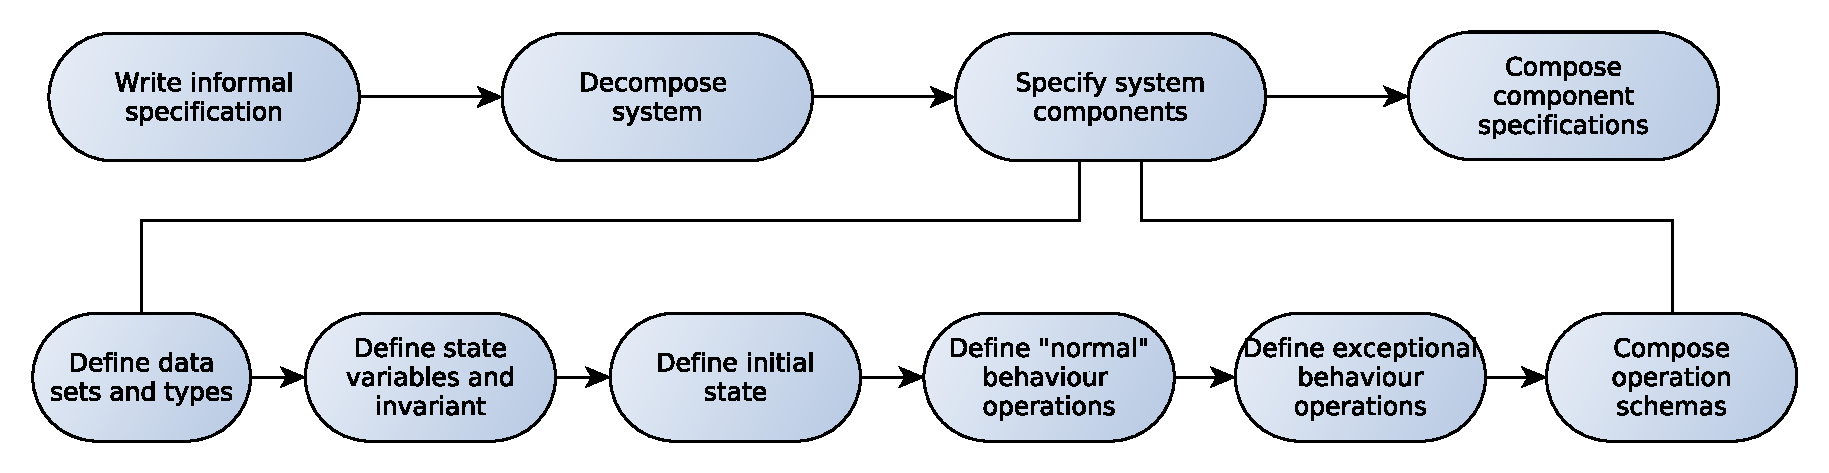
\includegraphics[scale=0.5]{\rootdir/specification/figures/specification-process}
\label{fig:specification:specification-process}
\caption{A process to develop a model-based specification of a system.}
\end{figure}

\section{Verification and validation}

As with any software engineering artifact, verification and validation (V\&V) are important. There are several techniques for V\&V of formal specifications:

\begin{enumerate}

 \item \emph{Animation}: Animation is the process of executing a specification with the intention of finding problems. The formal, unambiguous nature of specifications means that execution is often possible. However, because Sum (and many other formal specification languages) is built on first-order logic, not all specifications are executable. 

 We will look at animation of Sum specifications in the workshops.

 \item \emph{Model checking}: This is the process of attempting to execute every operation in every possible state of a system to show that certain properties hold; or more accurately, the find counterexamples of the properties. Model checking for model-based languages is difficult because the sheer number of states may be exponentially large, if not infinite. There is a lot of research around  the world looking at how to reduce the number of states for model checking while maintaining its soundness.

  If you have taken the subject \emph{Modelling Complex Software Systems}, you would used model checking to detect deadlock and to prove temporal logic properties of concurrency models.

 \item \emph{Review}: The specification can be subject to peer review, like any other document. This remains one of the most important and useful style of review for formal specification, despite advanced tools that can reason about them automatically.

 \item \emph{Proof}: Automated proof is the holy grail of formal specification. Proof is the most valuable of all techniques, because, unlike animation, model checking, reviews, and testing, if a property about a model can be proved, then we can say with strong conviction that it is true (although in reality, there is always the possibility that the proof itself is wrong!). 

\end{enumerate}

In this section, we discuss proof in more detail. This is not a major part of the subject, however, proof is an important motivation as to why practitioners adopt formal methods in software and systems engineering. Woodcock and Davies \cite{woodcock-using-z} present a far more thorough and valuable use of proof in specification. In this section, we discuss the implications of proof and present a trivial example.

\subsubsection*{The importance of proof}

If we have a specification of a system, then by reasoning about it using proof, we are likely to detect problems. If we have not started implementing the system, this provides us with an opportunity to find those problems before they become costly to fix. Further to this, the very process of constructing a proof can assist us in finding new requirements. That is, if we notice that we cannot prove a property about a system because some exceptional state has not been considered, we may need to add a requirement for this exceptional state. As Woodcock and Davies state: ``The practice of proof makes for better specifications''.

There is a commonly-held opinion that proof is not possible on large-scale systems. Industrial application of formal specification and proof shows this opinion to be wrong. Proof can be applied to real systems running in real environments, and can provide cost savings too. There are situations where proof is not relevant or necessary, but to high integrity systems especially, there are situations where it is desirable and almost necessary. There may be some situations where a sketch of a proof is sufficient. The trick in apply proof is to know which proofs are worth attempting, which are worth sketching, and which are worth leaving.

It is worth referencing the following quote:

\begin{quote}
``\emph{Things like even software verification, this has been the Holy Grail of computer science for many decades but now in some very key areas, for example, driver verification we're building tools that can do actual proof about the software and how it works in order to guarantee the reliability}." --- Bill Gates, Chairman of Microsoft, speaking at WinHEC 2002 in Seattle, Washington, USA.
\end{quote}

\subsubsection*{What can be proved?}

Proof is used in some high integrity systems for cases in which the outcome of failure is catastrophic; e.g.\ resulting in death or complete mission failure. The types of properties that can be proved vary, however, some interesting properties that have been proved about formal models include:

\begin{itemize}

 \item Proofs that certain security protocols cannot be cracked. More importantly, there have been cases of security protocols where proofs have demonstrated that they \emph{can} be cracked.

 The \emph{Needham-Schroeder Public-Key Protocol} is a protocol intended to provide mutual authentication between two parties communicating over a network, proposed by Roger Needham and Michael Schroeder in 1978. It was considered to be a failproof way to establish identity between two communicators, however, it was not until Gavin Lowe applied formal proof to the protocol in 1995 that it was discovered that the protocol failed to prevent ``man-in-the-middle'' attacks.

 \item Proofs about safety properties. Many safety-critical systems need to ensure certain safety properties hold. For example, railway signalling systems need to ensure that, given an intersection of tracks, at no stage will overlapping tracks both have non-red signals. That is, only one train will be allowed on the intersection at any time. These properties are specified a temporal logic properties, and it can be shown that a formal specification preserves these properties.

 \item In many life-critical systems, formal proof is applied to minimise the risk of causing harm or death. In many systems employed on NASA space missions, proof is applied to demonstrate that certain cases cannot go wrong. In particular, NASA has been known to reject entire proposals for systems on aerospace systems or life-support systems for astronauts unless model checking or proof have been used to demonstrate mission-critical properties (mainly around safety).

\end{itemize}

\subsubsection*{What can't proof do?}

It is important to say that if we ``prove'' our specification, then it is correct. When we do proofs about a formal specification, we are only proving that certain properties hold. We can say with some conviction that, if our proof can be discharged, then the property holds. However, this is only valuable if the property is correct. Further, we can do many proofs on a system, but omit an important one. Thus, a set of proofs is only as strong as the set of properties they show.

In most cases, proofs are not automated. That is, we cannot provide a specification and a property, and then have it proved. There are a large set of proofs for which this is possible, but there is another set for which it is currently not. The holy grail of theorem proving is exactly to prove things automatically, but for now, it remains a pipedream. For many logics, it has been proved that not all provable properties of the system can be automatically proved.

\subsubsection*{An example}

As a small example of how proof words, we'll return to the chemical storage system. 

\begin{example}

In the chemical storage system, the storage tank has a maximum limit, and if that limit is breached, serious safety consequences may result.
However, the overfilling problem is resolved using careful specification, and we can prove that the storage tank will not overflow, providing our specification is implemented correctly.

If we consider the \texttt{Fill} operation, it is broken into two parts: \texttt{FillOK} and \texttt{OverFill}. The \texttt{OverFill} operation does not add anything to the storage tank, so cannot cause it to overflow. This can be proved in a straightforward manner. The more challenging task is to show that the \texttt{FillOK} operation does not cause an overflow. So, we tackle this.

We know that the \texttt{FillOK} operation is only defined if the precondition is true. Therefore, the precondition forms the premise of our argument. What needs to be shown is that, if the precondition holds, then the resulting postcondition will not violate the safety property (the tank overflowing). Therefore, our proof has the following three components:

\begin{itemize}

 \item \emph{Precondition}: $contents + amount? \leq capacity$

 \item \emph{Postcondition}: $contents' = amount? + contents$

 \item \emph{Safety property}: $contents' \leq capacity$ (which is also the state invariant).

\end{itemize}

We can then structure our proof as follows:

\begin{center}
$Precondition \implies (Postcondition \implies Safety\ property)$
\end{center}

That is, if the precondition is true, then the postcondition implies that the safety property holds.

For the \texttt{FillOK} operation, this is straightforward to discharge. We have to prove:

\quad  $contents + amount? \leq capacity ~\implies$

\vspace{-2mm}

\quad\quad $(contents' = contents + amount? \implies contents' \leq capacity)$

Using the \emph{one-point rule}, we can replace all instances of \texttt{contents'} with \texttt{contents + amount?}: 

\quad  $contents + amount? \leq capacity \implies~$

\vspace{-2mm}

\quad\quad $(contents + amount? = contents + amount? \implies contents + amount? \leq capacity)$

The middle proposition $contents + amount? = contents + amount?$ is trivially true, so can be removed from the entire proposition, leaving:

\quad  $contents + amount? \leq capacity \implies contents + amount? \leq capacity $,

which is itself trivially true.

So, we have \emph{proved} that, for every possible state of the system, if the precondition holds, the storage container will not be filled beyond capacity. This is much stronger than throwing a million tests at it to see if we can find an input/state pair that violates it.

\end{example}

The above example is trivial in comparison to the types of proofs that are discharged on industrial scale systems, however, it illustrates how proof can be applied to a model-based specification.

Despite the small size, the proof required a few steps are several lines of text.  However, significant tool support is available for theorem proving. Using automated and interactive theorem provers, many large proofs can be discharged in a fairly straightforward manner, and the documentation of the proof can be generated automatically and stored digitally.


% LocalWords:  lifecycle Abrial Sommerville VDM statecharts PDF LMS
% LocalWords:  schemas nat powerset GivenType aboveskip sc FreeType
% LocalWords:  ModuleName dec pred linerange OperationName pre init
% LocalWords:  postconditions PrimaryColours forall emptyset structs
% LocalWords:  LargeSchema LeftSchema RightSchema PostFill GSM EF DF
% LocalWords:  EFs DFs mf df gsm ef dl dr iccid ddl ddr acm nia imsi
% LocalWords:  PINs PUK PUKs ALW CHV CICS el issubset GSMFiles chv lp
% LocalWords:  GSMSecurity SchemaName WinHEC Needham failproof FillOK
% LocalWords:  OverFill NewVariable OldVariable pipedream logics
% LocalWords:  FillTwice
